In Fig. \ref{fig:1.2.4_angle_py}, $RS$ is the median.  Hence, 
\begin{align}
	\vec S = \frac{\vec P + \vec Q}{2}
\end{align}
%
Hence, the equation of the median going through points $\vec S$ and $\vec R$ can be given as 
\begin{align}
	\vec x &= \vec R + \lambda \left(\vec S - \vec R\right)
	\\
	\vec x &= \myvec{4\\5} + \lambda \left(\myvec{0\\2} - \myvec{4\\5}\right)
	\\
	\vec x &= \myvec{4\\5} + \lambda \left(\myvec{-4\\-3}\right)
\end{align}
\begin{figure}[!ht]
	\centering
	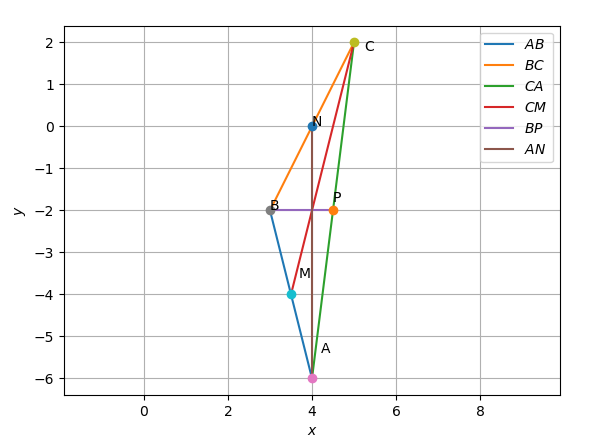
\includegraphics[width=\columnwidth]{./solutions/4/figures/triangle/triangle.eps}
	\caption{}
	\label{fig:1.2.4_angle_py}
\end{figure}
\begin{lstlisting}
solutions/4/codes/triangle/triangle.py
\end{lstlisting}
